% AsyncProof

\chapter{Asynchronous Two-Way Ranging Proof} % Main appendix title

\label{AsyncProof} % For referencing this appendix elsewhere, use \ref{AppendixA}

\section{Proof}
\begin{figure}
	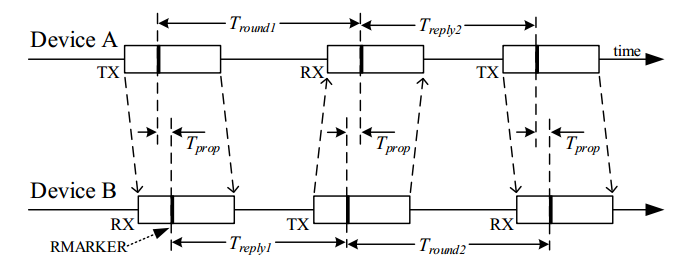
\includegraphics[width=\linewidth]{tprop.png}
	\caption{Double-sided Two-way ranging with three messages}
\end{figure}

We begin by assuming that the clock of one node is off by alpha ($\alpha$) and the other by beta ($\beta$), the key here was to find the time of flight in a virtual clock that would be the mean value of alpha and beta.
\\
\[ \alpha a = 2t + \beta c  \tag{1} \label{eq:1} \]
\[ \beta d = 2t + \alpha b  \tag{2} \label{eq:2} \]
\[ 1 = \frac{\alpha + \beta}{2} \]
\\
We simplify and solve for $\beta$:
\\
\[ \beta = 2 - \alpha  \tag{3} \label{eq:3} \]
\\
We then subsititute equation \eqref{eq:3} into equation \eqref{eq:1} and equation \eqref{eq:2}.
\\
\[ \alpha a = 2t + 2c - \alpha c  \tag{4} \label{eq:4} \]
\[ 2d - \alpha d = 2t + \alpha b  \tag{5} \label{eq:5} \]
\\
Isolate $\alpha$ for both equations \eqref{eq:4} and \eqref{eq:5} we get the following:
\\
\[ \alpha = \frac{2(t + c)}{a + c}  \tag{4.1} \label{eq:4.1} \]
\[ \alpha = \frac{2(d - t)}{b + d}  \tag{5.1} \label{eq:5.1} \]
\\
Setting \eqref{eq:4.1} and \eqref{eq:5.1} equal to each other we can solve for propagation time, t.
\\
\[ 2(t + c)(b +d) = 2(d - t)(a + c)\]
\[ tb + td +bc + dc = da + dc - ta - tc \]
\[ t(b + d + a + c) = da - bc\]
\[ t = \frac{da-bc}{a + b + c + d}  \tag{6} \label{eq:6} \]
\\
